\chapter{Template chapter}

\label{ChapterTemplate} % For referencing the chapter elsewhere, use \ref{Chapter1} 

\section{Images}

\subsection{Standard image}

\begin{figure}[H]
\centering
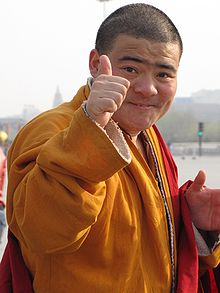
\includegraphics[width=8cm]{Figures/yeh_monk.jpg}
\decoRule
\caption[img-name]{Yeh Monk! \parencite{cf_1.2_eigentaste}.}
\label{fig:monkeh}
\end{figure}

\subsection{Side-by-side}

\begin{figure}[H]
  \centering
  \begin{minipage}[b]{0.45\textwidth}
    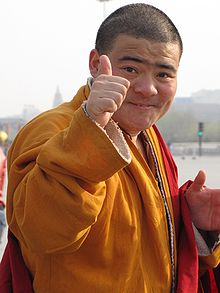
\includegraphics[width=\textwidth]{Figures/yeh_monk.jpg}
    \caption[Monk1]{Monk 1.}
  \end{minipage}
  \hfill
  \begin{minipage}[b]{0.45\textwidth}
    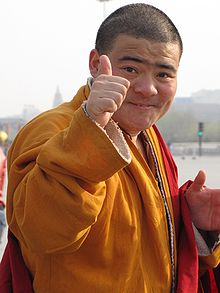
\includegraphics[width=\textwidth]{Figures/yeh_monk.jpg}
    \caption[Monk2]{Monk 2.}
  \end{minipage}
\end{figure}

\section{lists}

\subsection{Itemize}
\begin{itemize}
\item What levels of accuracy can be achieved in the positional accuracy of features calculated using photogrammetric intersection of Street View images?
\item What are the limiting factors with regards to improving positional accuracy?
\end{itemize}

\subsection{Enumerate}
\begin{enumerate}
\item What is the accuracy achieved for a detected feature within a Street View image using a convolutional neural network?
\item What is the best level of accuracy achieved for positioning common features found in multiple Street View images?
\item When combining the two components (image classifier and intersection) what is the final positional accuracy of features?
\end{enumerate}

\section{Tables}

\begin{table}[H]
\caption[Classifier Results]{The first 50 images were bins while the second 50 were in the unknown category}
\label{tab:classifier_results}
\centering
\begin{tabular}{c l c | c l c}
\toprule
\textbf{Image} & \textbf{Label} & \textbf{Score} & \textbf{Image} & \textbf{Label} & \textbf{Score} \\
\midrule
1 & Bin & 0.99510 & 1 & Unknown & 0.99416 \\
2 & Bin & 0.97168 & 2 & Unknown & 0.99246 \\
3 & Bin & 0.99604 & 3 & Unknown & 0.97483 \\
\bottomrule\\
\end{tabular}
\end{table}
